\chapter{Introduction to Elder Topology}

\textit{This chapter presents the topological framework that connects abstract Elder spaces to practical applications through realization mappings. We develop phase-coherent manifolds that bridge theoretical structures with observable phenomena in specific domains. The topological properties of Elder spaces—including their phase-preserving homomorphisms, spectral invariants, and stratification—explain fundamental mechanisms like resonance and cross-domain transfer. This mathematical foundation establishes Elder Theory as a rigorous formalism with precise guarantees for knowledge representation and transfer capabilities.}

\section{Topological Structure}

Elder spaces possess a natural topology that arises from their algebraic structure and phase properties.

\begin{definition}[Elder Topology]
The topology on an Elder space is based on the product topology of the parameter space and phase space. The basic open sets include both parameter proximity and phase alignment considerations.
\end{definition}

\begin{theorem}[Topological Properties]
An Elder space with its natural topology forms a well-behaved mathematical space that supports continuity of the knowledge transfer operations essential to the theory.
\end{theorem}

\begin{definition}[Resonance Manifold]
A subset $\mathcal{M}$ of an Elder space is a resonance manifold if it represents a collection of elements that maintain consistent phase relationships when parameter values change. These manifolds provide the mathematical structure for knowledge transfer across domains.
\end{definition}

\begin{theorem}[Gravitational Stratification]
Every Elder space can be organized into gravitational field regions that represent different levels of knowledge abstraction:
\begin{equation}
\mathcal{E} = \bigcup_{k=0}^{d} \mathcal{S}_k
\end{equation}
where each $\mathcal{S}_k$ represents a collection of related knowledge structures at a particular gravitational field strength corresponding to a level of abstraction.
\end{theorem}

\begin{figure}[ht]
\centering
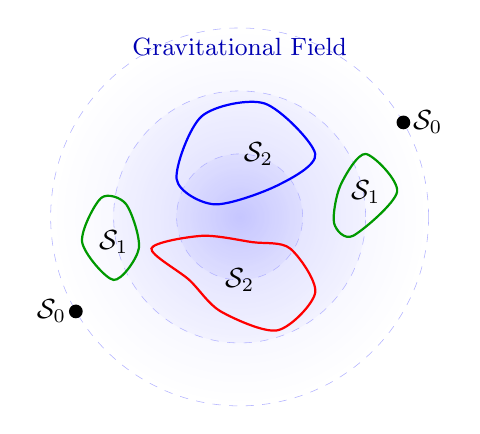
\begin{tikzpicture}[scale=0.8]
% Draw gravitational field using gradient shading
\shade[inner color=blue!20, outer color=white, opacity=0.4] (0,0) circle (3);
\shade[inner color=blue!30, outer color=blue!10, opacity=0.3] (0,0) circle (2);
\shade[inner color=blue!40, outer color=blue!20, opacity=0.3] (0,0) circle (1);

% Add subtle field lines for gravitational effect
\foreach \r in {1,2,3}
  \draw[blue!30, dashed, very thin] (0,0) circle (\r);

\draw[blue, thick] plot [smooth cycle] coordinates {(0.6,0.5) (1.2,1.0) (0.4,1.8) (-0.6,1.6) (-1.0,0.6) (-0.4,0.2)};
\node at (0.3,1.0) {$\mathcal{S}_2$};

\draw[red, thick] plot [smooth cycle] coordinates {(-1.4,-0.5) (-0.8,-1.0) (-0.3,-1.5) (0.6,-1.8) (1.2,-1.2) (0.8,-0.5) (0.2,-0.4) (-0.6,-0.3)};
\node at (0,-1.0) {$\mathcal{S}_2$};

\draw[green!60!black, thick] plot [smooth cycle] coordinates {(-2.2,0.3) (-2.5,-0.4) (-2.0,-1.0) (-1.6,-0.5) (-1.8,0.2)};
\node at (-2.0,-0.4) {$\mathcal{S}_1$};

\draw[green!60!black, thick] plot [smooth cycle] coordinates {(1.8,-0.3) (2.5,0.4) (2.0,1.0) (1.6,0.5) (1.5,-0.1)};
\node at (2.0,0.4) {$\mathcal{S}_1$};

\filldraw (2.6, 1.5) circle (0.1) node[right] {$\mathcal{S}_0$};
\filldraw (-2.6, -1.5) circle (0.1) node[left] {$\mathcal{S}_0$};

% Add gravitational field label
\node[font=\small, text=blue!70!black] at (0,2.7) {Gravitational Field};
\end{tikzpicture}
\caption{Stratification of Elder space as resonance manifolds within a gravitational field. Each layer ($\mathcal{S}_0$, $\mathcal{S}_1$, $\mathcal{S}_2$) represents knowledge structures at different levels of abstraction and field strengths.}
\label{fig:elder-stratification}
\end{figure}

This stratification is important for understanding the organization of knowledge in the Elder Theory framework, as each layer corresponds to information with similar structural properties and abstraction levels.

\section{Domain Mappings}

Domain mappings connect abstract knowledge in Elder spaces to concrete applications across different fields of study.

\begin{definition}[Domain Mapping]
A domain mapping connects knowledge within the Elder framework to practical applications in a specific field or domain, allowing theoretical principles to be applied to real-world problems.
\end{definition}

\begin{theorem}[Knowledge Transfer]
The Elder framework facilitates knowledge transfer across domains through mappings that preserve essential relationships and structural patterns:
\begin{enumerate}
    \item Conservation of structure: Key relationships are maintained across domain boundaries
    \item Adaptability: Knowledge can be applied to new domains while preserving essential patterns
    \item Phase alignment: Related concepts across domains naturally align through resonance
    \item Hierarchical preservation: Knowledge maintains its hierarchical organization across domains
\end{enumerate}
\end{theorem}

This approach enables knowledge discovered in one field to be meaningfully applied to different domains while preserving the core structural patterns and relationships.

\section{Phase Properties}

The phase properties of Elder spaces provide important insights into how knowledge components interact and align.

\begin{definition}[Phase Alignment]
Phase alignment in Elder Theory refers to the synchronization of related knowledge components across different domains, enabling effective knowledge transfer and integration.
\end{definition}

\begin{theorem}[Knowledge Resonance]
When knowledge structures from different domains share underlying principles, they exhibit resonance properties that facilitate their integration:
\begin{enumerate}
    \item Common patterns become amplified through phase alignment
    \item Domain-specific details that don't align are naturally filtered
    \item Integrated knowledge maintains essential structural relationships
    \item Cross-domain insights emerge from the resonance patterns
\end{enumerate}
\end{theorem}

\begin{theorem}[Knowledge Transfer Properties]
The Elder framework facilitates knowledge transfer through structural correspondence:
\begin{enumerate}
    \item Similar structures in different domains can be mapped to each other
    \item The mapping preserves essential relationships between components
    \item Knowledge from one domain can guide learning in another domain
\end{enumerate}
\end{theorem}

\section{Hierarchical Knowledge Structure}

The hierarchical organization of Elder spaces is central to understanding knowledge transfer across domains.

\begin{theorem}[Hierarchical Organization]
The Elder-Mentor-Erudite hierarchy represents knowledge at different levels of abstraction:
\begin{enumerate}
    \item Elder level: Universal principles and patterns that apply across all domains
    \item Mentor level: Domain-specific knowledge that organizes related concepts
    \item Erudite level: Task-specific implementations and applications
\end{enumerate}
\end{theorem}

\begin{corollary}[Cross-Domain Transfer]
Knowledge can be transferred between domains when:
\begin{enumerate}
    \item Common patterns are identified at the Elder level
    \item Corresponding domain-specific implementations are mapped
    \item Essential relationships and structures are preserved during transfer
\end{enumerate}
\end{corollary}

This approach enables efficient knowledge transfer between domains by leveraging shared underlying principles while adapting to domain-specific requirements.

\section{Resonance Principles}

The Elder framework uses resonance as a fundamental mechanism for connecting related knowledge across domains.

\begin{definition}[Knowledge Resonance]
Knowledge resonance occurs when related concepts across different domains show structural similarities that can be leveraged for knowledge transfer and integration.
\end{definition}

\begin{theorem}[Resonance Properties]
Knowledge resonance in the Elder framework has several important properties:
\begin{enumerate}
    \item Similar knowledge structures naturally align and reinforce each other
    \item Resonant knowledge becomes more accessible and influential in the system
    \item Learning naturally gravitates toward coherent knowledge structures
    \item Cross-domain insights emerge from resonant patterns
\end{enumerate}
\end{theorem}

These resonance principles explain how the Elder-Mentor-Erudite system discovers meaningful connections across domains, providing a foundation for effective knowledge transfer and integration.

\section{Learning Dynamics}

The Elder framework includes important principles about how knowledge evolves and develops over time.

\begin{theorem}[Pattern Recognition]
Learning in the Elder framework exhibits systematic pattern recognition:
\begin{enumerate}
    \item Recurring patterns across domains are detected and emphasized
    \item Common structural relationships become incorporated into higher-level knowledge
    \item Domain-specific variations are treated as contextual adaptations
\end{enumerate}
\end{theorem}

\begin{theorem}[Knowledge Evolution]
As learning progresses in the Elder framework, knowledge structures evolve in predictable ways:
\begin{enumerate}
    \item From specific instances to general principles
    \item From isolated concepts to connected knowledge networks
    \item From domain-specific applications to cross-domain patterns
\end{enumerate}
\end{theorem}

These learning dynamics explain how the Elder-Mentor-Erudite framework naturally develops increasingly sophisticated and transferable knowledge representations over time.

The conceptual framework established in this chapter provides the foundation for understanding how the Elder Theory approach connects abstract principles to concrete applications, explaining the system's core capabilities of efficient knowledge representation, hierarchical organization, and cross-domain transfer.